
\documentclass[preprint,12pt]{elsarticle}

\usepackage[spanish]{babel}
\usepackage{amssymb}
\usepackage{graphicx}
\usepackage{lineno}

\usepackage{abstract} % Allows abstract customization
\renewcommand{\abstractnamefont}{\normalfont\bfseries} % Set the "Abstract" text to bold
\renewcommand{\abstracttextfont}{\normalfont\small\itshape} % Set the abstract itself to small italic text

\usepackage[utf8]{inputenc}
\usepackage{url}
\usepackage{natbib}

\begin{document}
	
	\begin{frontmatter}
		\title{\huge UNIVERSIDAD PRIVADA DE TACNA \\}
		\title{INFORME DE LABORATORIO N°1 SONARQUBE }
		\author{
			Alumno: Rafael Martín Callata Flores \\
			Curso: Calidad y Pruebas de Software \\
			Docente: Patrick Cuadros Quiroga
		}
		\address{Tacna, Perú}
	\end{frontmatter}


%%INICIO Objetivos
\section{Objetivos}

%%----------------------------------------------------------------------------------------------------------------------------------------------------------
	\subsection{\textbf{General}}
	Implementar la prueba de calidad con sonarqube de un proyecto paso a paso.
	\subsection{\textbf{Específicos}}
	\begin{itemize}
		\item realizar la instalación del SonarQube
		\item realizar pruebas del codigo fuente de un proyecto
		\item realizar la configuracion del SonarQube
		\item realizar las instalaciones de programas necesarios para las pruebas de calidad 
	\end{itemize}
%%FIN Objetivos
%%INICIO Objetivos
\section{\textbf{Materiales}}
	\begin{itemize}
		\item WINDOWS 10 PRO
		\item DOCKER DESKOP
		\item SONARQUBE
	\end{itemize}
%%FIN Objetivos
%%INICIO Desarrollo del Trabajo
\section{Desarrollo Del Trabajo}	
\begin{itemize}
	%%----------------------------------------------------------------------------------------------------------------------------------------------------------
	\item Descargar SonarQube
	\begin{center}
		docker pull sonarqube \\
		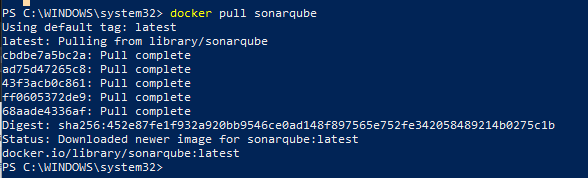
\includegraphics[width=15cm]{./imagen/descargasonarqube}
	\end{center}
	%%----------------------------------------------------------------------------------------------------------------------------------------------------------
	\item Ejecutar una instancia de SonarQube
	\begin{center}
	docker run -d --name sonarqube -p 9000:9000 sonarqube \\
	Nota: para eliminar una instancia previa puede utilizar el comando: docker rm -f sonarqube \\
	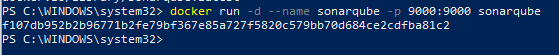
\includegraphics[width=15cm]{./imagen/instanciasonarqube}
	\end{center}
	%%----------------------------------------------------------------------------------------------------------------------------------------------------------
	\item Ingresar al portal con las credenciales
	\begin{center}
	http://localhost:9000/ \\
	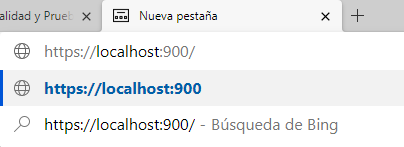
\includegraphics[width=8cm]{./imagen/urlportal}
\end{center}
\begin{center}
	presionar el botón Log in para logearse \\
	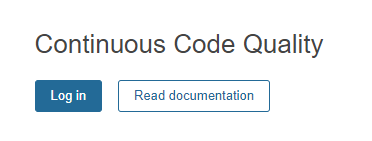
\includegraphics[width=9cm]{./imagen/ingresoregistro}
\end{center}
\begin{center}
	user: admin \\
	pass: admin \\
	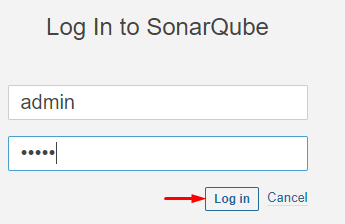
\includegraphics[width=10cm]{./imagen/logearportal}
	\end{center}
	%%----------------------------------------------------------------------------------------------------------------------------------------------------------
	\item Crear una nueva aplicación con el nombre aplicacionNetCore
	\begin{center}
			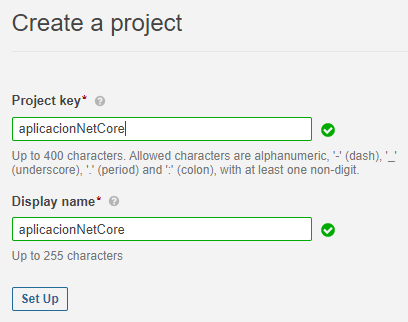
\includegraphics[width=8cm]{./imagen/crearproyecto}
	\end{center}
	%%----------------------------------------------------------------------------------------------------------------------------------------------------------
	\item Generar el token de la nueva aplicación aplicacionNetCore
	\begin{center}
		primero ingresamos el nombre del proyecto \\
		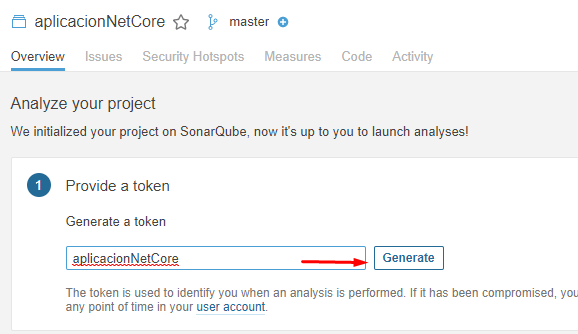
\includegraphics[width=8cm]{./imagen/generartoken}
	\end{center}
\begin{center}
	luego generamos el token \\
	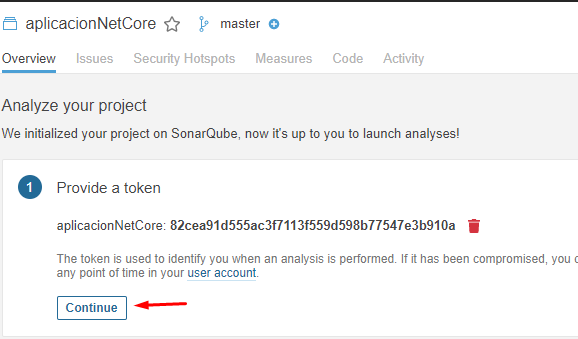
\includegraphics[width=8cm]{./imagen/tokengenerado}
\end{center}
	%%----------------------------------------------------------------------------------------------------------------------------------------------------------
	\item Descargar NetCore e instalar

	\begin{center}
			https://dotnet.microsoft.com/download/dotnet-core/thank-you/sdk-3.1.300-windows-x64-installer \\
		descargamos el ejecutable \\
		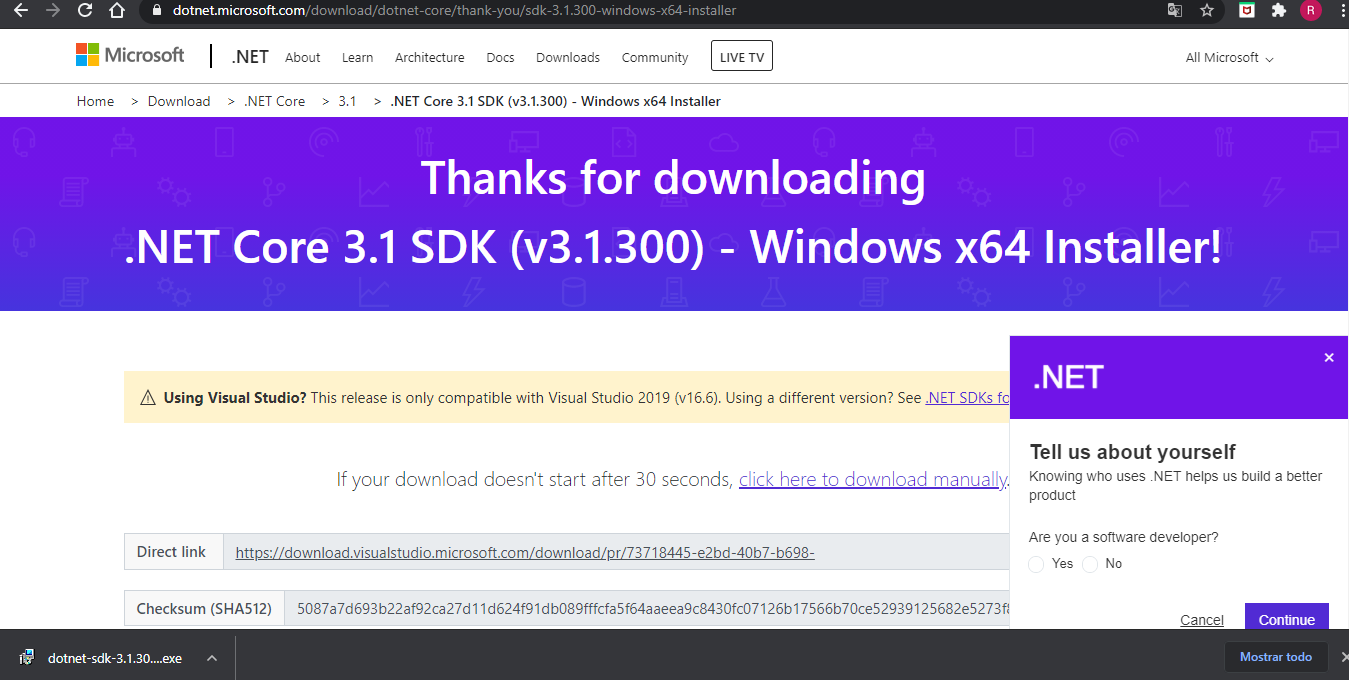
\includegraphics[width=7cm]{./imagen/ejecutable}
	\end{center}
	\begin{center}
	  ejecutamos el programa NetCore \\
		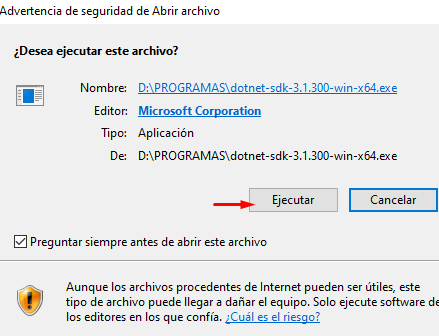
\includegraphics[width=8cm]{./imagen/ejecutarNetCore}
	\end{center}
\begin{center}
	instalamos el programa NetCore \\
	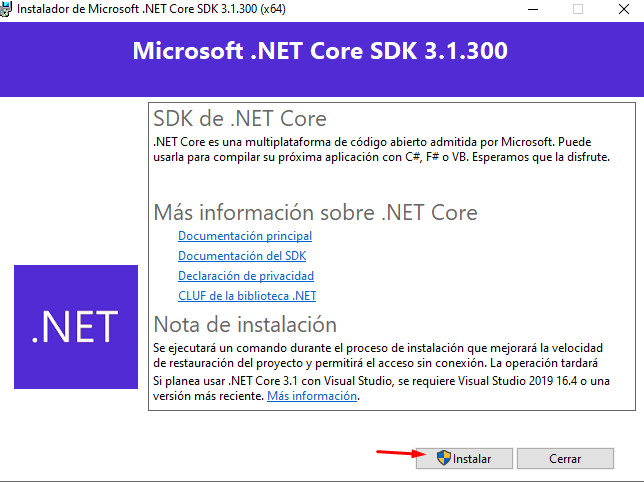
\includegraphics[width=8cm]{./imagen/instalarNetCore}
\end{center}
%%----------------------------------------------------------------------------------------------------------------------------------------------------------
\item En un terminal ejecutar e instalar sonar-scanner

\begin{center}
	dotnet tool install --global dotnet-sonarscanner \\
	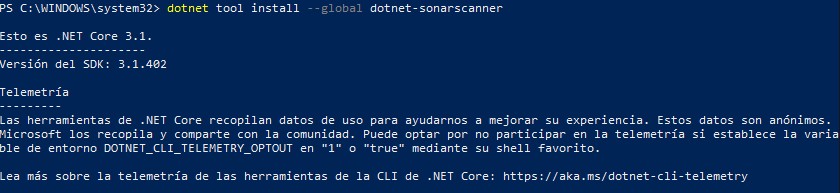
\includegraphics[width=10cm]{./imagen/sonarscanner}
\end{center}

%%----------------------------------------------------------------------------------------------------------------------------------------------------------
\item En un terminal, acceder a una ruta donde creara una nueva aplicación

\begin{center}
	dotnet new sln -o aplicacionNetCore \\
	ejecutamos este comando \\
	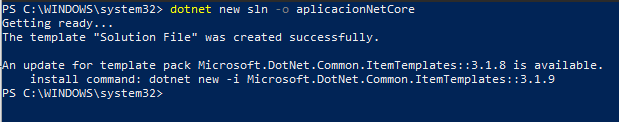
\includegraphics[width=10cm]{./imagen/ruta1}
\end{center}
\begin{center}
	cd aplicacionNetCore \\
	ejecutamos este comando \\
	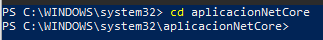
\includegraphics[width=7cm]{./imagen/ruta2}
\end{center}
\begin{center}
	dotnet new console \\
	ejecutamos este comando \\
	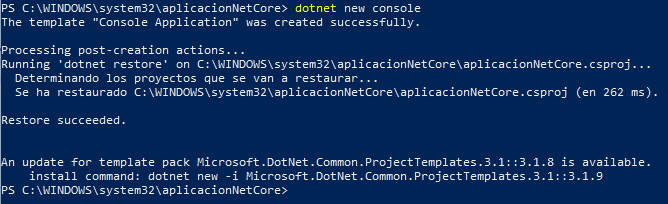
\includegraphics[width=11cm]{./imagen/ruta3}
\end{center}
\begin{center}
	dotnet sln aplicacionNetCore.sln add aplicacionNetCore.csproj \\
	ejecutamos este comando \\
	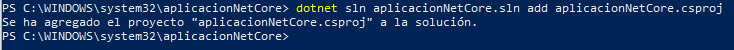
\includegraphics[width=11cm]{./imagen/ruta4}
\end{center}
%%----------------------------------------------------------------------------------------------------------------------------------------------------------
\item En el mismo terminal, iniciar la sesión de revisión de sonarqube

\begin{center}
	dotnet sonarscanner begin /d:sonar.host.url="http://localhost:9000" /d:sonar.login=admin /d:sonar.password=admin /k:”aplicacionNetCore” \\
	ejecutamos este comando \\
	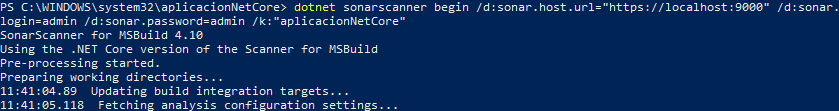
\includegraphics[width=9cm]{./imagen/iniciarsesion}
\end{center}
%%----------------------------------------------------------------------------------------------------------------------------------------------------------
\item Compilar la aplicacion
\begin{center}
	dotnet build \\
	ejecutamos este comando \\
	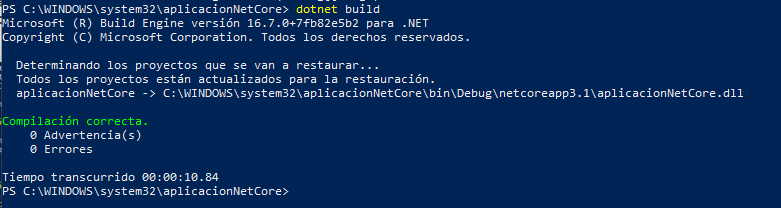
\includegraphics[width=10cm]{./imagen/build}
\end{center}
%%----------------------------------------------------------------------------------------------------------------------------------------------------------
\item Cerrar la sesion
\begin{center}
	dotnet sonarscanner end /d:sonar.login=admin /d:sonar.password=admin \\
	ejecutamos este comando \\
	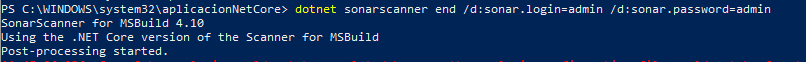
\includegraphics[width=10cm]{./imagen/cerrarsesion}
\end{center}
%%----------------------------------------------------------------------------------------------------------------------------------------------------------
\item Resultado
\begin{center}
	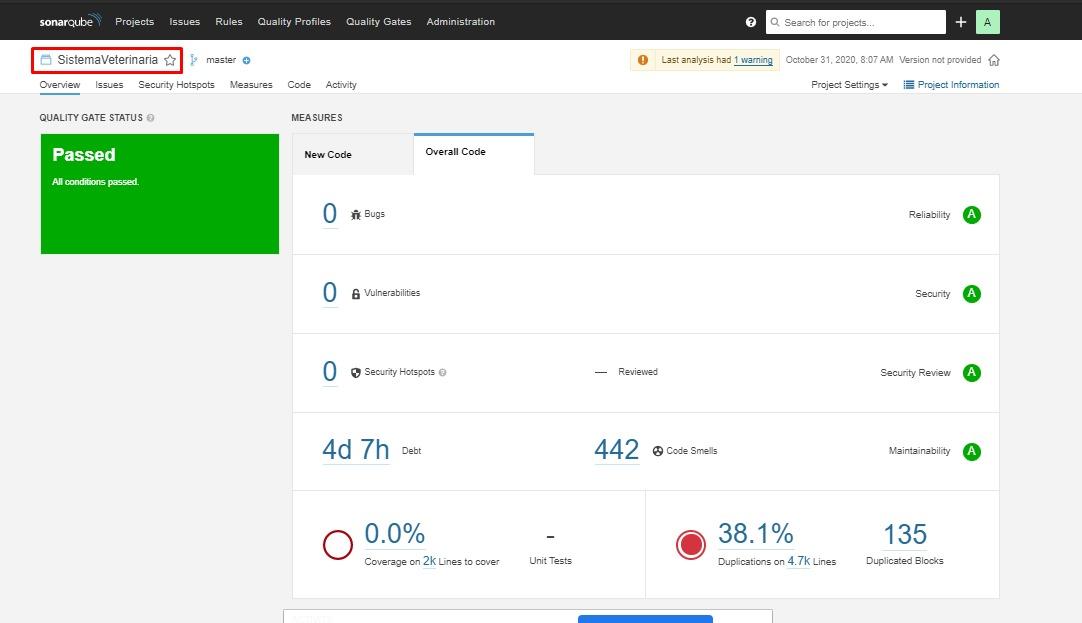
\includegraphics[width=10cm]{./imagen/resultado}
\end{center}


\end{itemize}
%%FIN Desarrollo del Trabajo
%%INICIO Conclusiones
\section{Conclusiones de SonarQube }

\begin{itemize}
	
	\item Duplicacion de codigo \\
	Sonarqube nos proporciono un 38.1 de código duplicado, este detecto partes de nuestro software que se asemejan. La duplicación de código es generalmente considerada una señal de estilo de programación pobre, un buen desarrollo está más asociado a la reutilización del mismo. Es por eso que debemos aspirar a mejor nuestra forma de programar.
	
	\item CodeSmells  	\\
	Sonarqube nos proporciono un total de 442 de codesmells. En este caso la letra A, significa que no tenemos alguna deuda tecnica, sin embargo si tuvieramos una letra E esto significaria que el código fuente del programa  indique posiblemente un problema más profundo. Pero en este caso nos refiere que el proyecto presenta un level moderable de codesmells.
	
	\item La calidad de código suele decirse que es un atributo interno de calidad, dado que no se hace visible al usuario. Pero llega un momento en el cual este atributo de calidad pasa de ser interno a externo, y esto se da cuando el hecho de tener modificar el código para hacer un cambio lleva mucho más tiempo del que debería. Con el fin de verificar la calidad interna de un sistema se suelen hacer análisis de código con SonarQube o herramientas similares. 
	
\end{itemize}

%%FIN Conclusiones
\end{document}